\section{Business Value}
\label{sec:value}

\subsection{Framing the headline number}
The current result is that \textbf{about 21--25\% of reserved online-inference GPU-hours} are reclaimable while keeping under-provisioning at or below the \textbf{5\% safety constraint} ($U \le 5\%$). The 21\% end is the measured matched-risk result on unseen clusters (20.8\% A1, 21.9\% A3); the 25\% end is the upper end of the current estimate range and should be treated as provisional until E9 removes the history-feature leakage. Three tiers keep the claim honest:

\begin{table}[h]
\centering\small
\caption{Savings tiers, from opportunity to risk-constrained policy.}
\label{tab:tiers}
\begin{tabularx}{\linewidth}{@{}p{3.3cm}cL@{}}
\toprule
Tier & Reclaimed & What it assumes \\
\midrule
Opportunity (upper) & 25\% & Provisional upper estimate; Model A only; perfect packing of freed slices. \\
Opportunity (measured) & 21\% & Matched $U=5\%$ on unseen clusters; Model A only; perfect packing. \\
A+B policy, no risk cap & 11.4\% & Long-running pods; Model B re-scores each shrink; risk rises 36.0\%\ra37.8\%. \\
A+B policy, +2-point cap & 3.4\% & Only shrinks Model B deems near-risk-neutral; mostly extrapolated sizes. \\
\bottomrule
\end{tabularx}
\end{table}

\subsection{Lower GPU cost}
Per 1{,}000 reserved GPUs there are $1{,}000 \times 8{,}760 = 8.76$M GPU-hours per year. Reclaiming a share $r$ frees $r \times 8.76$M GPU-hours, or equivalently $r \times 1{,}000$ GPUs of steady capacity. We price this at three illustrative on-demand rates: $\approx$\$1/GPU-h for A10-class cards (approximate; ASI's online fleet is dominated by A10, L20 and H20 parts), \$3.43 for A100 80GB (AWS p4de per GPU), and \$3.90 for H100 (AWS P5 after the June 2025 price cut~\cite{aws2025price}, from secondary aggregators). Owned fleets have lower effective rates than on-demand, so these are upper-range translations.

\begin{table}[h]
\centering\small
\caption{Annual value per 1{,}000 reserved inference GPUs. GPU-hours in millions; dollars in millions per year. Scale linearly with fleet size.}
\label{tab:value}
\begin{tabular}{@{}lcccccc@{}}
\toprule
Tier & Reclaimed & GPU-h freed & GPUs freed & @\$1.00 & @\$3.43 & @\$3.90 \\
\midrule
Opportunity (upper) & 25\% & 2.19 & 250 & \$2.19 & \$7.51 & \$8.54 \\
Opportunity (measured) & 21\% & 1.84 & 210 & \$1.84 & \$6.31 & \$7.17 \\
A+B, no cap & 11.4\% & 1.00 & 114 & \$1.00 & \$3.43 & \$3.89 \\
A+B, +2-pt cap & 3.4\% & 0.30 & 34 & \$0.30 & \$1.02 & \$1.16 \\
\bottomrule
\end{tabular}
\end{table}

\begin{figure}[h]
\centering
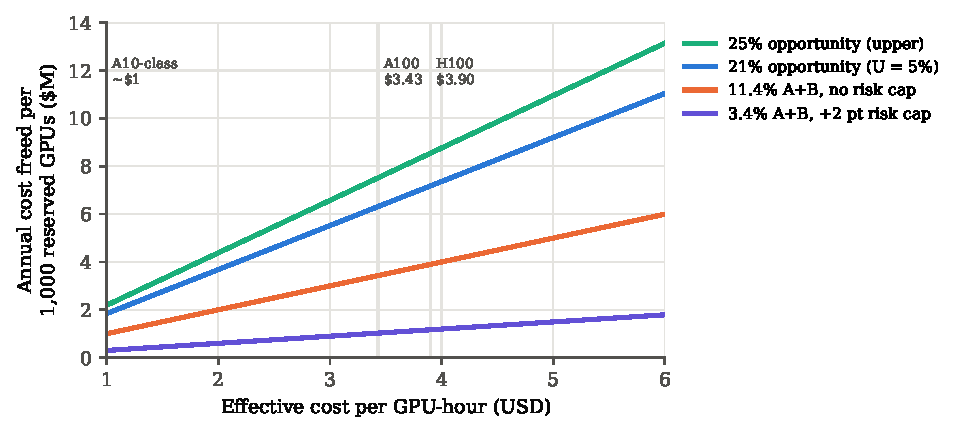
\includegraphics[width=0.8\linewidth]{figures/fig_value.pdf}
\caption{Annual cost freed per 1{,}000 reserved GPUs as a function of effective GPU-hour price, for each savings tier.}
\label{fig:value}
\end{figure}

\noindent For capital planning, \cref{eq:util} gives the same story: reclaiming 21\% of reservations is equivalent to raising effective utilization of the reserved pool by a factor of $1/(1-0.21) \approx 1.27$, so a fleet sized for today's demand could absorb $\approx$27\% more of the same workload before buying GPUs.

\subsection{Less idle capacity}
ASI reports online-inference median SM utilization of 6\% and an allocation ratio of 68\% for high-priority work before SpotGPU~\cite{li2026asi}. Right-sizing at admission shrinks reservations \emph{before} they become idle headroom. Because recommendation pods hold most of the reclaimable capacity (33--43\% for rec-with-history), the most direct win is consolidating recommendation serving onto fewer GPUs.

\subsection{Faster job completion}
Capacity freed from over-reserved inference does not disappear; it returns to the pool used by preemptible training, offline inference and development jobs. In ASI, low-priority jobs already run on harvested capacity, and making that capacity \emph{reserved-free} rather than \emph{borrowed} reduces evictions; ASI's preemption-cost-aware victim selection alone cut low-priority completion time by 24\%~\cite{li2026asi}. We do not estimate a JCT gain from the trace; the simulator (E10) would.

\subsection{More reliable provisioning}
Model B addresses a separate cost: 46\% of D2 pods fail to become ready, and each failed placement temporarily occupies GPUs. Zhang and Liao~\cite{zhang2026ineffective} show readiness-aware ordering cuts ineffective occupancy from 43.64\% to 27.15\% on an Alibaba trace. A calibrated Model B used as a veto keeps right-sizing from trading GPU-hours for failed placements, and used on its own could steer risky pods (large, low-priority, scarce GPU type, busy server) to safer placements.

\subsection{Caveats on value}
Realized savings will be lower than the opportunity tiers because (i) freed fractions must be packable onto shared GPUs, and ASI shows sharing is rare due to weak isolation; (ii) $U$ is not a latency SLO; (iii) the A+B tiers rely on Model B extrapolating to unseen sizes. The value table should be read as the ceiling that justifies building the mechanism, not as a forecast.
